% 逻辑主线: 终端设备隐藏的巨大数据与算力潜力如何解决当前数据枯竭和算力集中问题?

% 第4章:海量终端设备带来的AI新机遇
% \section{Opportunities and Benefits}
\section{Scaling Beyond Limits: Opportunities from Edge Devices}
\label{sec:opportunities}
% \section{New Opportunities through Edge Devices}
% The Hidden Potential from Edge Devices.  
% - 统计终端设备量。
% - 统计终端设备量。
% 4.1 海量终端数据: 冰山下的巨大能量
\subsection{Massive Data from Edges}
\label{subsec:edge_data}
% - 公共数据只占全量数据的冰山一角
% - 单个设备数据存储量很大
% - 全球活跃终端设备的规模有多大?(数十亿设备是否足够弥补当前公共数据枯竭)
% xxxxxx- 哪些类型的数据可以从终端设备中挖掘?(对话,纯文本等)输入法
% - 本地化数据的质量相比公共数据如何?
% \begin{figure}
%     \centering
% 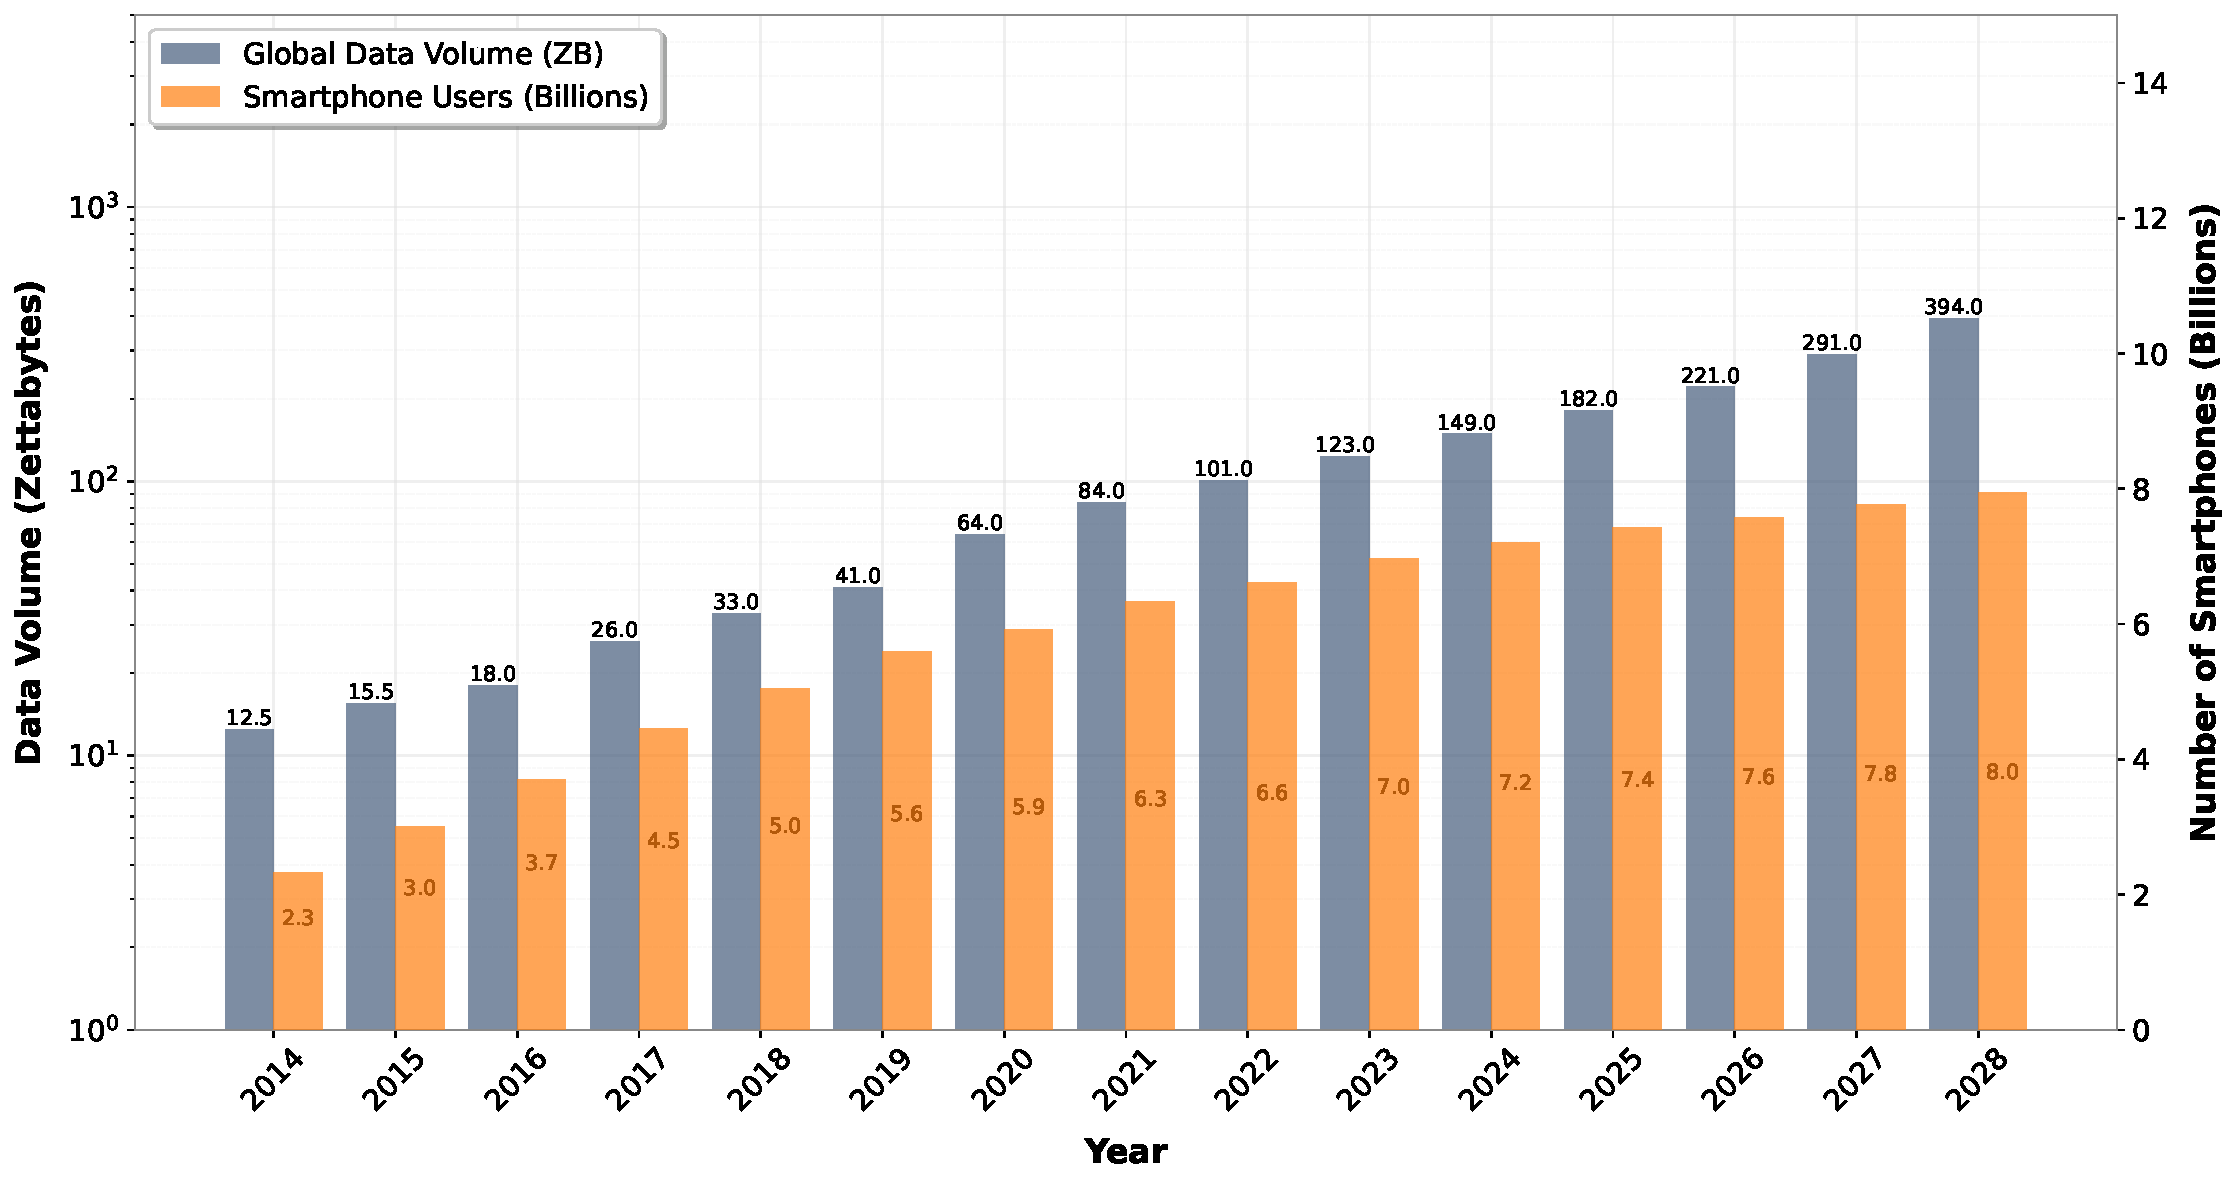
\includegraphics[width=\linewidth]{./figs/trends_bar.pdf}
%     \caption{Global Data Volume and Smartphone Users Growth from 2014 to 2028.}
%     \label{fig:proj}
% \end{figure}

% \begin{figure}
%     \centering
% 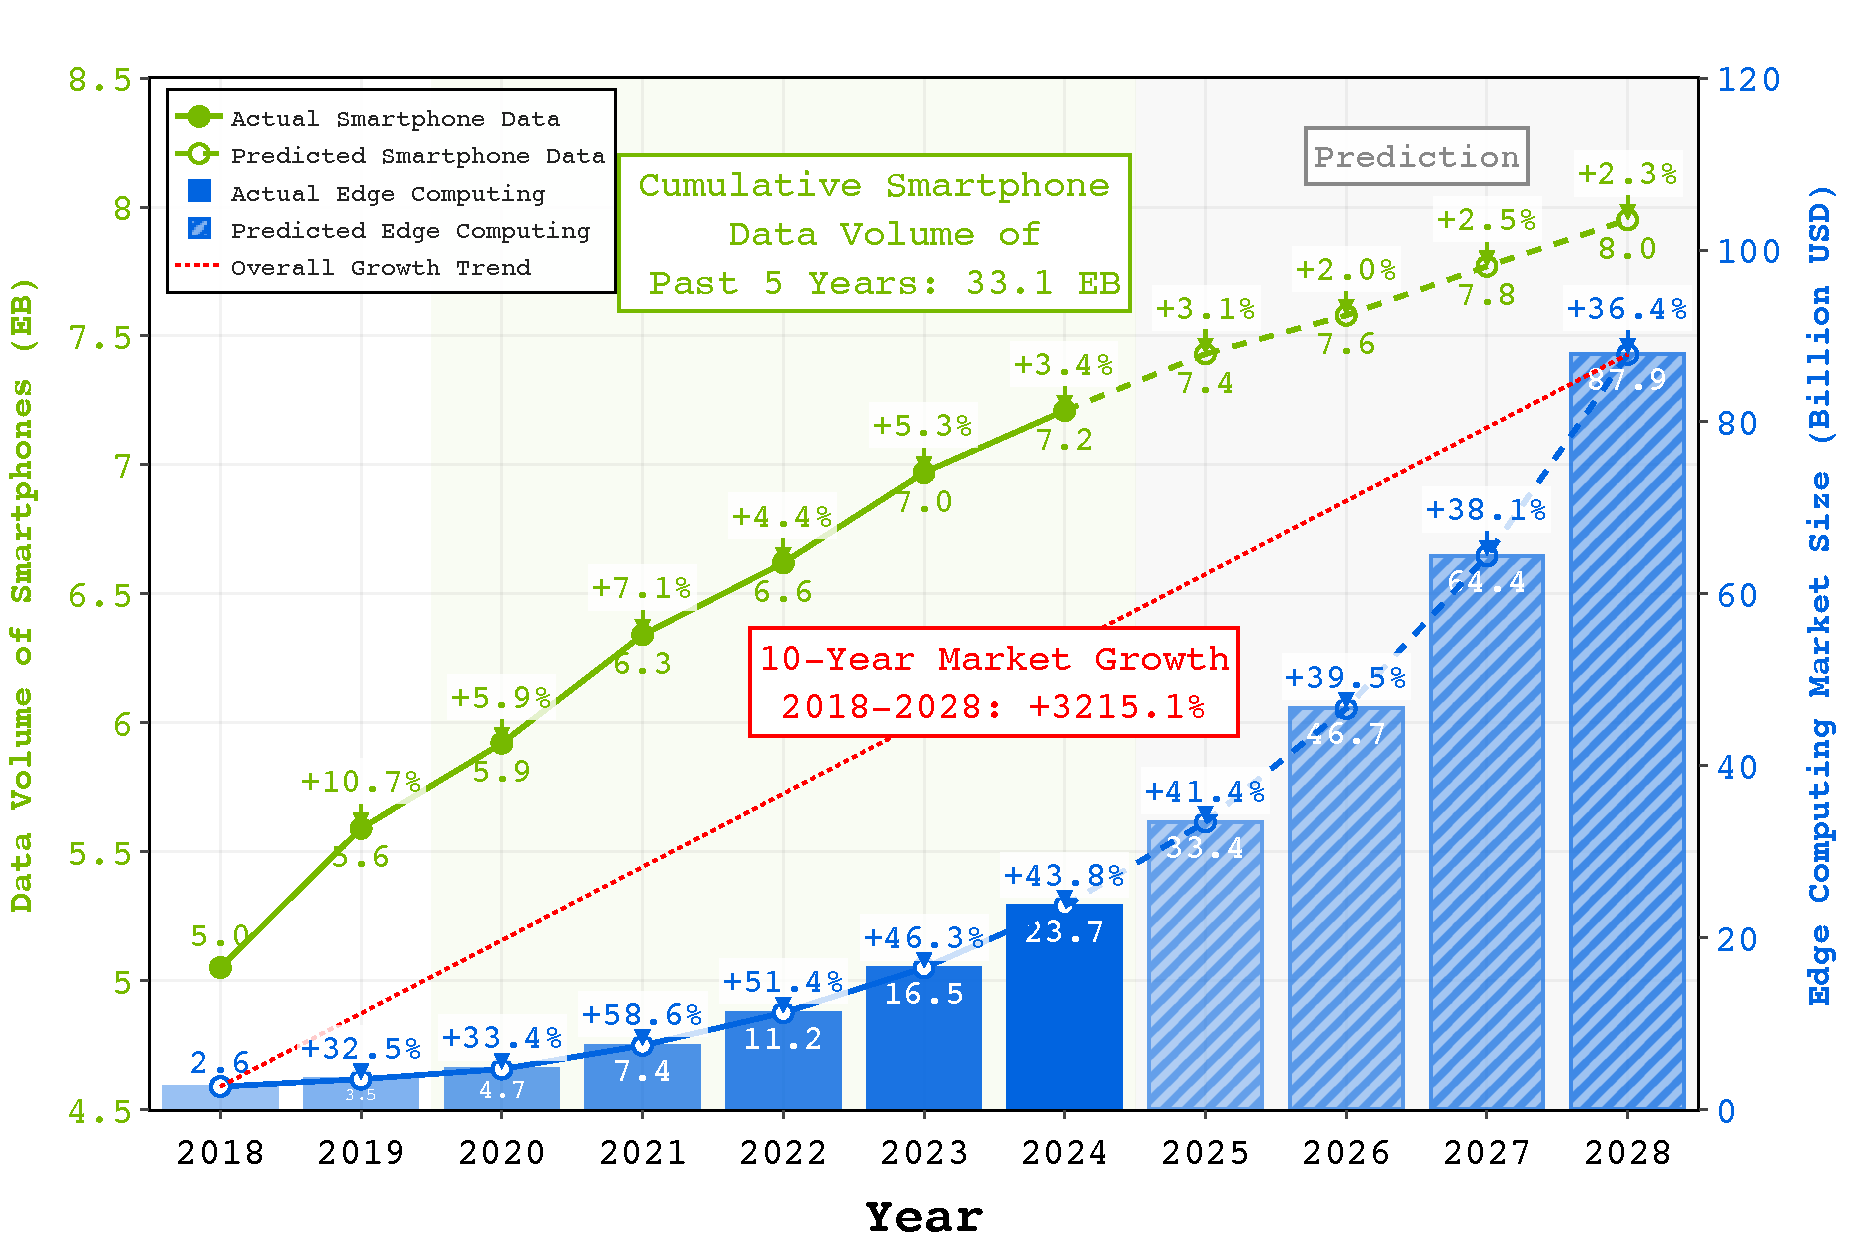
\includegraphics[width=\linewidth]{./figs/edge_and_smartphone.pdf}
%     \caption{Smartphone users growth with edge computing market size (right) from 2014 to 2028.}
%     \label{fig:proj}
% \end{figure}

\begin{figure*}[htbp]
    \centering
    \begin{minipage}[t]{0.49\linewidth}
        \centering
        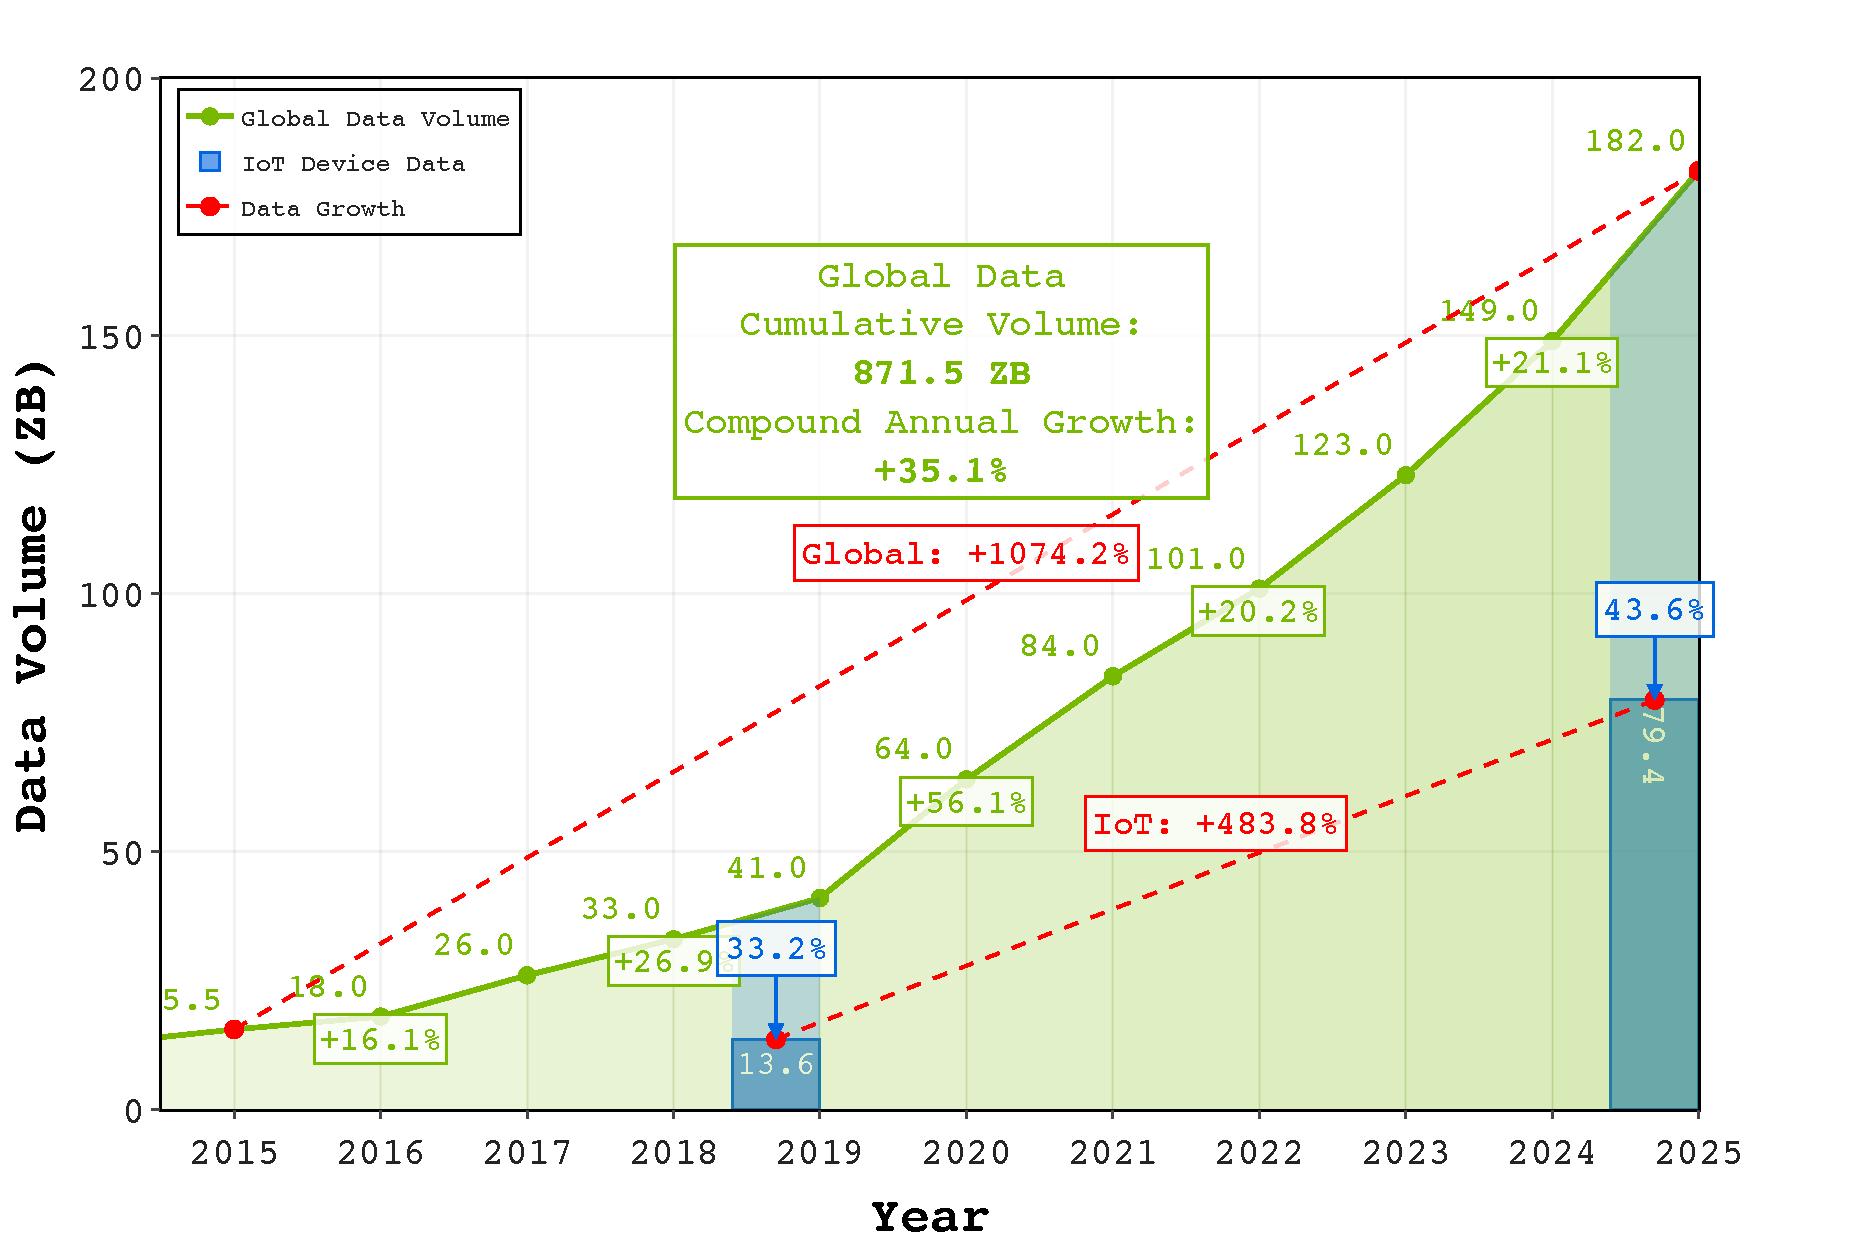
\includegraphics[width=\linewidth]{./figs/iot_data_contribution.pdf}
\vspace{-20pt}
        \caption{Global data volume from 2014 to 2025 and IoT device data volume in 2015 and 2025. (Data sources: Global data volume from \cite{statista_global_2023}; IoT device data volume from \cite{statista_iot_2023}.)}
    \label{fig:global_data}
    \end{minipage}
    \hfill
    \begin{minipage}[t]{0.49\linewidth}
        \centering
        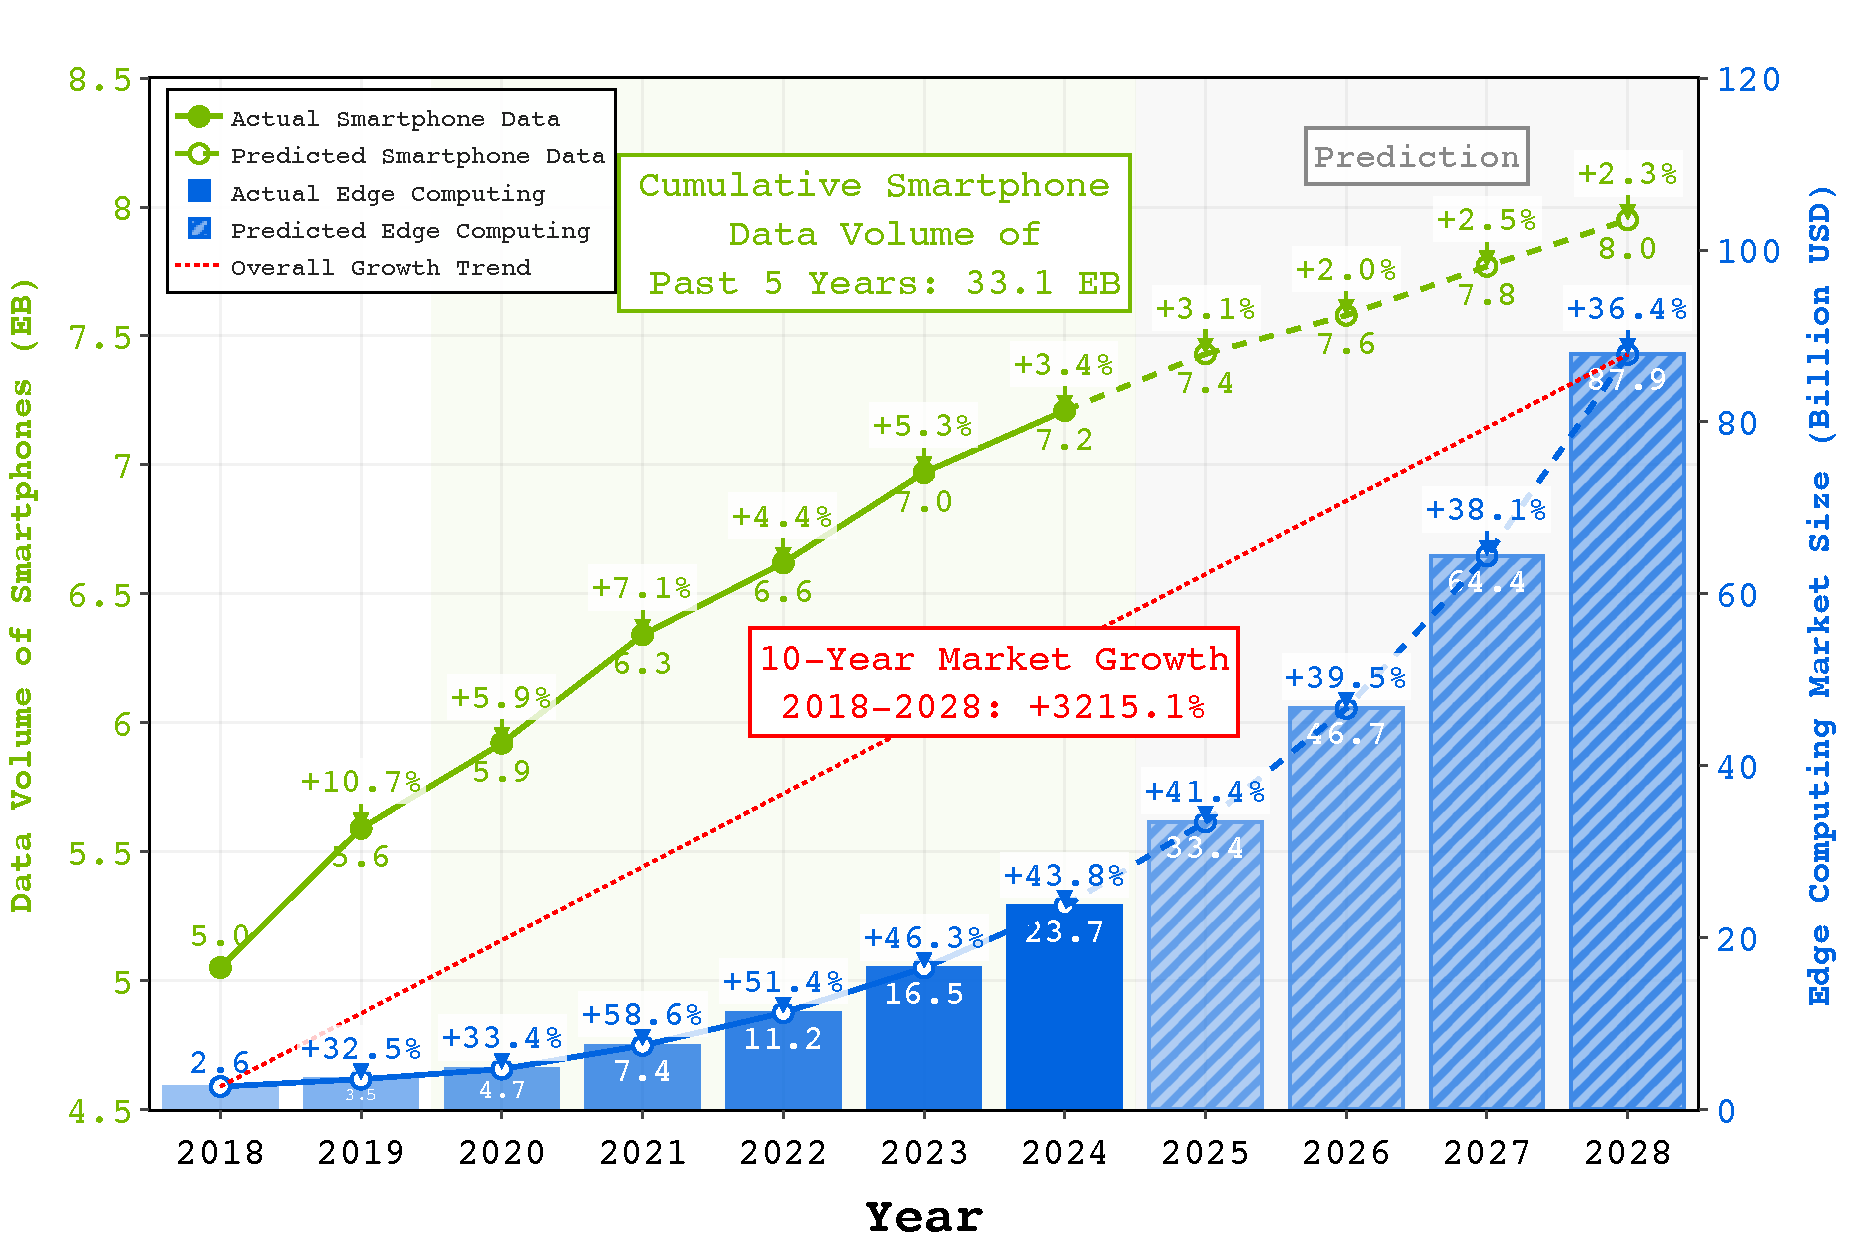
\includegraphics[width=\linewidth]{./figs/edge_and_smartphone.pdf}
\vspace{-20pt}

        \caption{Smartphone data volume with edge computing market size (right) from 2018 to 2028. (Data sources: Edge computing market \cite{grandview_edge_2023}; Smartphone data volume derived from the number of smartphones \cite{bankmycell_smartphone_2023}.)}
    \label{fig:smartphone}
    \end{minipage}
    
\end{figure*}


% As mentioned in \S\ref{subsec:data_exhaustion}, in addition to synthetic data, edge data is considered another important avenue for addressing the issue of data exhaustion. 
% While publicly available data is vast, it represents only the tip of the iceberg in terms of total data volume. In contrast, the amount of data generated by edge devices (such as smartphones, tablets, and IoT devices) is significantly larger and exhibits high diversity and personalization. 
% According to estimates in the literature, the number of active edge devices worldwide has reached billions, with each device generating several to tens of gigabytes of data daily~\cite{villalobos2022trends}. This data encompasses various types, including user conversations, input method records, and sensor data, offering immense potential value.

% The types of data generated by edge devices are highly diverse, primarily including user conversation data, input method data, and sensor data. Instant messaging applications (such as WhatsApp and WeChat) generate hundreds of billions of messages daily, with each message containing an average of 4-5 tokens~\cite{rosenfeld2018whatsapp}. 
% These data not only include textual information but may also encompass multimedia content such as voice, images, and videos. Smartphone input methods record users' typing habits, frequently used vocabulary, and language styles, which can help models better understand the diversity and complexity of natural language. Additionally, sensor data (such as location, temperature, and motion data) generated by IoT devices (e.g., smart home devices and wearables) can provide additional contextual information for models, particularly in multimodal tasks.

% Compared to public data, local data has significant advantages in terms of quantity and quality. First, in terms of quantity, the scale of local data far exceeds that of public data. Taking social media platforms as an example, Facebook generates approximately 10 trillion tokens of text data annually, while Twitter and Instagram generate around 1.5 trillion and 800 billion tokens, respectively~\cite{villalobos2022trends}. This data is not only massive in scale but also highly diverse and real-time, making it a valuable resource for training language models. In contrast, public datasets (such as Common Crawl) have a total volume of about 400 trillion tokens, and their growth rate is relatively slow~\cite{hoffmann2022training}.

% Second, in terms of quality, local data typically exhibits higher personalization and contextual relevance. Although public data undergoes some cleaning and filtering, its content is often generic and lacks deep understanding of specific users or scenarios. In contrast, local data (such as user conversations and input method records) captures users' personalized language habits, cultural backgrounds, and real-time needs, thereby providing richer contextual information for models. For example, input method data reflects users' frequently used vocabulary and expressions, while social media data includes users' interests, emotions, and social network information. Such high-quality data can help models better adapt to diverse application scenarios, improving their generalization capabilities and user experience.

% However, the utilization of local data also faces several challenges. First, privacy concerns are a major obstacle. Data on edge devices often contains sensitive user information, and how to effectively utilize this data while protecting user privacy is an urgent issue. Second, data quality and standardization are also critical challenges. Local data is often fragmented and of inconsistent quality, making effective cleaning and standardization a technical hurdle. Finally, legal and ethical issues constrain the use of local data. Using local data for model training may pose legal risks, particularly regarding user privacy and data ownership.

% Despite these challenges, the potential of local data cannot be overlooked. Through technologies such as federated learning, it is possible to utilize data from edge devices for model training without compromising user privacy~\cite{konevcny2016federated}. Moreover, social media companies (such as Meta and Twitter) have begun exploring the possibility of using their own data for model training. For example, Meta's Llama series of models partially leverages user-generated content from Facebook and Instagram for training~\cite{touvron2023llama}. This "self-sustaining" model not only alleviates the issue of data exhaustion but also enhances the personalization and localization capabilities of models.

% Therefore, the utilization of edge data and social media data holds promise as an important supplement to address the issue of data exhaustion, especially as publicly available data becomes increasingly scarce. Through technological innovation and privacy protection measures, edge data and social media data can provide a sustainable source of data for model training.

As discussed in §~\ref{subsec:data_exhaustion}, edge data represents a crucial alternative to synthetic data in addressing the challenge of data exhaustion. Edge data refers to the data generated by edge devices at or near the source of data generation, which typically remains private and localized rather than being publicly accessible. Edge devices encompass a wide range of equipment including Internet of Things (IoT) sensors, smartphones, wearables, industrial controllers, and other smart devices that process data at the network edge. The global data ecosystem exhibits significant bifurcation: publicly available data constitutes merely the tip of the iceberg, while data generated by edge devices demonstrates superior strategic value both in terms of growth rate and high quality.

\paragraph{Edge-generated data is explosively growing.} 
% By 2025, it is projected that over 80\% of global data will be generated directly at the edge, rather than in traditional centralized data centers \cite{seagate_rethinkdata_2020}. This shift highlights a fundamental transformation in how data is created, processed, and utilized across industries.
As illustrated in Figure~\ref{fig:global_data}, the global data volume is projected to reach 182 ZB by 2025~\cite{statista_global_2023}, with a particularly pronounced growth in edge-generated data. The data generated by IoT devices is anticipated to increase from 13.6 ZB in 2019 to 79.4 ZB in 2025~\cite{statista_iot_2023}, elevating its share of the global data volume from 33.2\% to 43.6\%. Over the period from 2015 to 2025, the global data volume exhibited a compound annual growth rate (CAGR) of 35.1\%, resulting in an overall increase of 1074.2\% and a cumulative total of 871.5 ZB. IoT device data experienced a growth of 483.8\% from 2019 to 2025. This trend underscores the increasingly central role of edge-generated data in the global data ecosystem.
Beyond IoT devices, smartphones, as a critical source of edge-side data, are also contributing to the steady rise in data volume. As depicted in Figure~\ref{fig:smartphone}, the estimated smartphone data volume is projected to grow from 5 EB in 2018 to 8 EB by 2028
\footnote{These numbers are estimated based on an average user data generation of 1 GB per device. For detailed estimation methodology, refer to Appendix \ref{app:smartphone_ethod}.}. 
This exponential growth is closely aligned with the rapid expansion of the edge computing market, which is forecasted to surge from \$5.5 billion in 2019 to \$87.9 billion by 2028, representing a remarkable growth rate of 3215.1\%. The burgeoning edge computing market has further catalyzed the generation and processing of edge-side data, reinforcing its significance in the broader data landscape.
\vspace{-0.5cm}
\begin{insights}
    \textbf{Insight:} The smartphone data volume of the past 5 years (before 2025) is projected to reach approximately 33.1 EB, with unique advantages in privacy and real-time context, demonstrating the massive data potential of edge for AI model training.
\end{insights}
   
% To put this into perspective, the total volume of global data is expected to surpass 181 ZB annually by 2025 \cite{statista_global_2023}. This rapid growth is further fueled by the proliferation of IoT devices and connected technologies. As illustrated in Figure \ref{fig:global_data}, IoT devices alone are projected to account for 43.6\% of global data volume by 2025, marking a significant increase from their contribution of 33.2\% just six years prior. Meanwhile, as shown in Figure \ref{fig:smartphone}, smartphone data volume is projected to grow steadily from 3.5 EB in 2029 to 7.8 EB by 2028\footnote{Estimated using 1GB average data generation per device. See Appendix \ref{app:smartphone_ethod} for details.}, showcasing a consistent upward trajectory.
% The growth in data generation is paralleled by the expansion of the edge computing market, which is forecasted to rise from 5.5 billion in 2019 to 64.4 billion by 2028 \cite{grandview_edge_2023}, reflecting the widespread adoption of edge-centric architectures. 
% In summary, the immense volume of edge data with its rapid growth trajectory, establishes a promising foundation for pretraining at the edge.

\paragraph{Edge-generated data is of high quality.} 
Beyond its impressive quantity, edge data possesses several qualitative advantages that make it particularly valuable for model pretraining.
First, edge data exhibits superior \textit{diversity} across multiple dimensions. It encompasses a wide variety of data types from IoT devices, mobile interactions, and personal devices, covering different domains, languages, and user behaviors. This natural diversity provides richer training signals compared to curated public datasets \cite{nayak2024review}. 
Second, edge data demonstrates strong \textit{real-time capability}. Unlike public datasets, which are often updated infrequently, edge devices continuously generate fresh data with low latency \cite{cavliwireless_edgecomputing}, offering more up-to-date and relevant training samples.
Third, edge data offers enhanced \textit{personalization} characteristics. It enables real-time interactions and context-aware recommendations by leveraging local data such as location and device behavior. This allows for highly relevant and adaptive personalization that can dynamically adjust to user preferences \cite{xenonstack_edge_ai_2023}.
Fourth, edge data exhibits enhanced \textit{context awareness} due to the proximal positioning of edge devices to data sources, enabling the capture of fine-grained contextual information often absent in public datasets. For instance, wearable devices collect synchronized activity and location data, providing high-fidelity behavioral patterns that preserve temporal and spatial context.

\vspace{-0.1cm}
In conclusion, edge data with its explosive growth
\footnote{
\citet{idc_seagate_dataage_2019,seagate_rethinkdata_2020} provide a more comprehensive overview of the global data volume, but we cannot access the statistics data. 
We appreciate any suggestions for better statistical data sources.
}
and superior qualitative characteristics, is a valuable resource for model pretraining. Its diversity, real-time nature, personalization, and rich context make it an ideal foundation for developing robust and adaptable large-scale models, enhancing their ability to serve real-world applications effectively.



% Fourth, edge data provides superior \textbf{contextual completeness}, as evidenced by smart device interactions achieving 97\% contextual reasoning accuracy~\cite{llama2023}. This rich contextual information enables models to learn more comprehensive semantic relationships. 
% These characteristics - natural diversity, timely updates, diverse language patterns, and rich contextual information - make edge data an invaluable resource for enhancing the quality and effectiveness of large language model pretraining, particularly in capturing real-world language usage and user behaviors.


% \textbf{High quality of Edge-generated data.} Firstly, edge data is highly diverse. It comes from a wide variety of sources such as IoT devices, mobile phones, and wearable sensors. This diversity provides a more comprehensive and detailed view of the real-world scenarios. For example, in a smart city application, data from traffic cameras, weather stations, and air quality monitors can be combined to provide a holistic understanding of the urban environment. Secondly, edge data is more timely. Edge devices can process and analyze data in real-time or near-real-time, which is crucial for applications that require immediate responses. For instance, in an industrial automation setting, data from sensors on machinery can be used to detect faults and trigger maintenance actions before they lead to significant downtime. Thirdly, edge data is more context-aware. Edge devices are often located close to the data source, which allows them to capture context-specific information that may be lost in public data. For example, a wearable device can capture data about a user's physical activity and location, providing a more accurate picture of their behavior.

% Compared to public data, edge data demonstrates quality advantages across three dimensions: (1) \textbf{Real-time capability}: Social platform data latency typically remains under 500ms (Meta internal benchmarks), while public datasets usually update on cycles exceeding 6 months; (2) \textbf{Personalization}: The n-gram distribution in input method records shows significant user specificity, with Jensen-Shannon divergence 37\% higher than public corpora~\cite{touvron2023llama}; (3) \textbf{Contextual completeness}: Sensor data from smart home devices forms multimodal associations with user voice commands, enabling dialogue systems to achieve 97\% contextual reasoning accuracy~\cite{llama2023}. These characteristics make edge data crucial for enhancing model domain adaptability---Meta's Llama series models achieved a 12.3\% improvement in F1 score for personalization tasks by incorporating Instagram user-generated content (UGC)~\cite{touvron2023llama}.

% \textbf{Diversity of Edge-generated data.} Edge data has transcended traditional textual boundaries to form a comprehensive spectrum of multimodal sensory data: (1) \textit{Communication data}: Instant messaging applications (such as WhatsApp and WeChat) generate over 100 billion messages daily, with each message containing an average of 4-5 semantic units~\cite{rosenfeld2018whatsapp}; (2) \textit{Behavioral data}: Input method records capture user input patterns across over 200 language variants and personalized expression characteristics~\cite{tisi2023}; (3) \textit{Environmental data}: Biosensor data from smart wearables is growing at 41\% annually, with each device generating 1.2GB of physiological metrics daily~\cite{seagate2025}. This data not only vastly exceeds public datasets (Common Crawl's total volume is approximately 400 trillion tokens, with annual growth <5\%~\cite{hoffmann2022training}) but also possesses unique spatiotemporal correlations---smartphone location data combined with social media LBS information can construct user behavior profiles accurate to meter-level precision~\cite{gartner2025}.





% 4.2 海量终端算力: 云端下的巨大动力
\begin{figure*}[htbp]
    \centering
    \begin{minipage}[t]{0.49\linewidth}
        \centering
        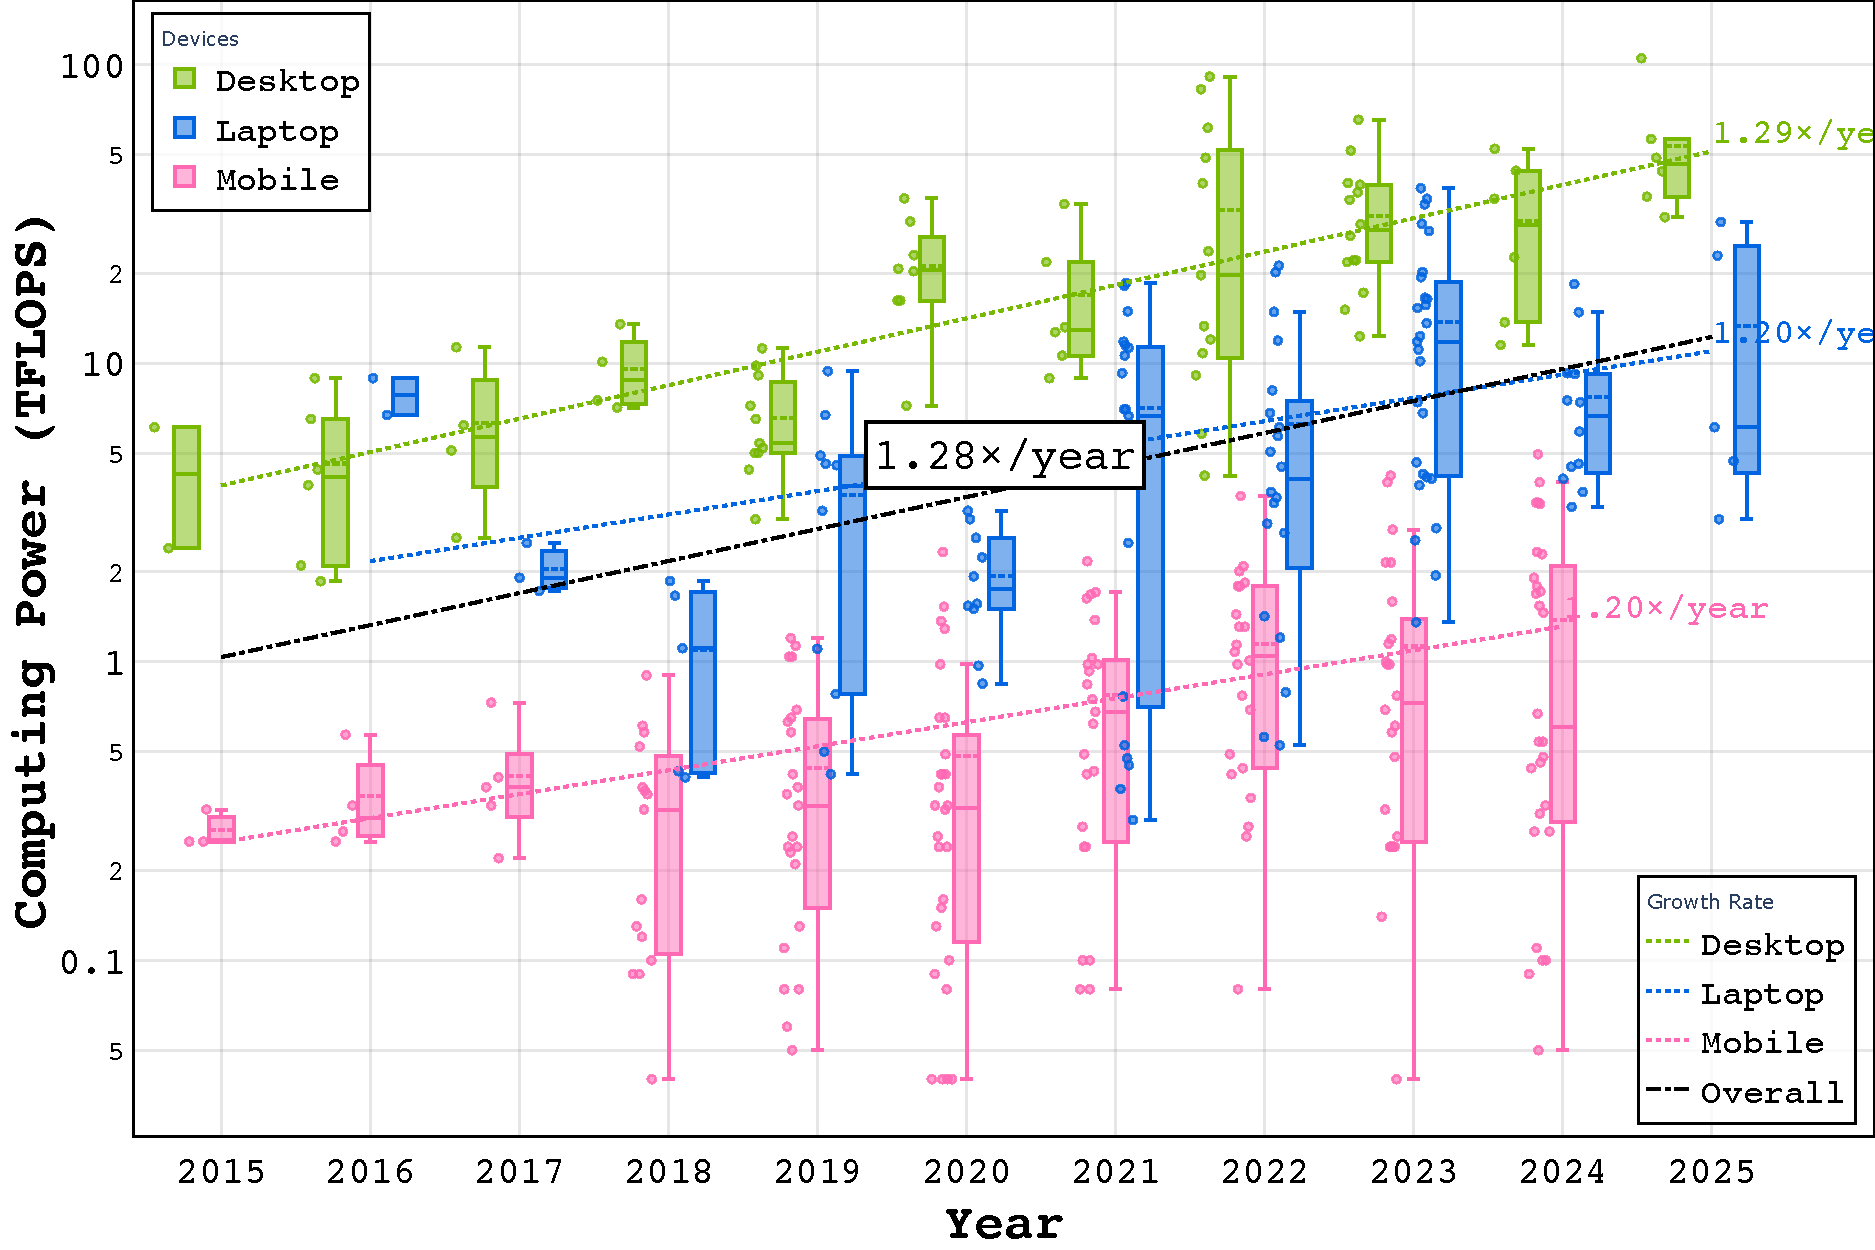
\includegraphics[width=\linewidth]{./figs/edge_compute_trend.pdf}
        \vspace{-20pt}
        \caption{Edge Computing Power Evolution Trend. (Data source: \cite{nanoreview2025}).}
        \label{fig:edge_trend}
    \end{minipage}
    \hfill
    \begin{minipage}[t]{0.49\linewidth}
        \centering
        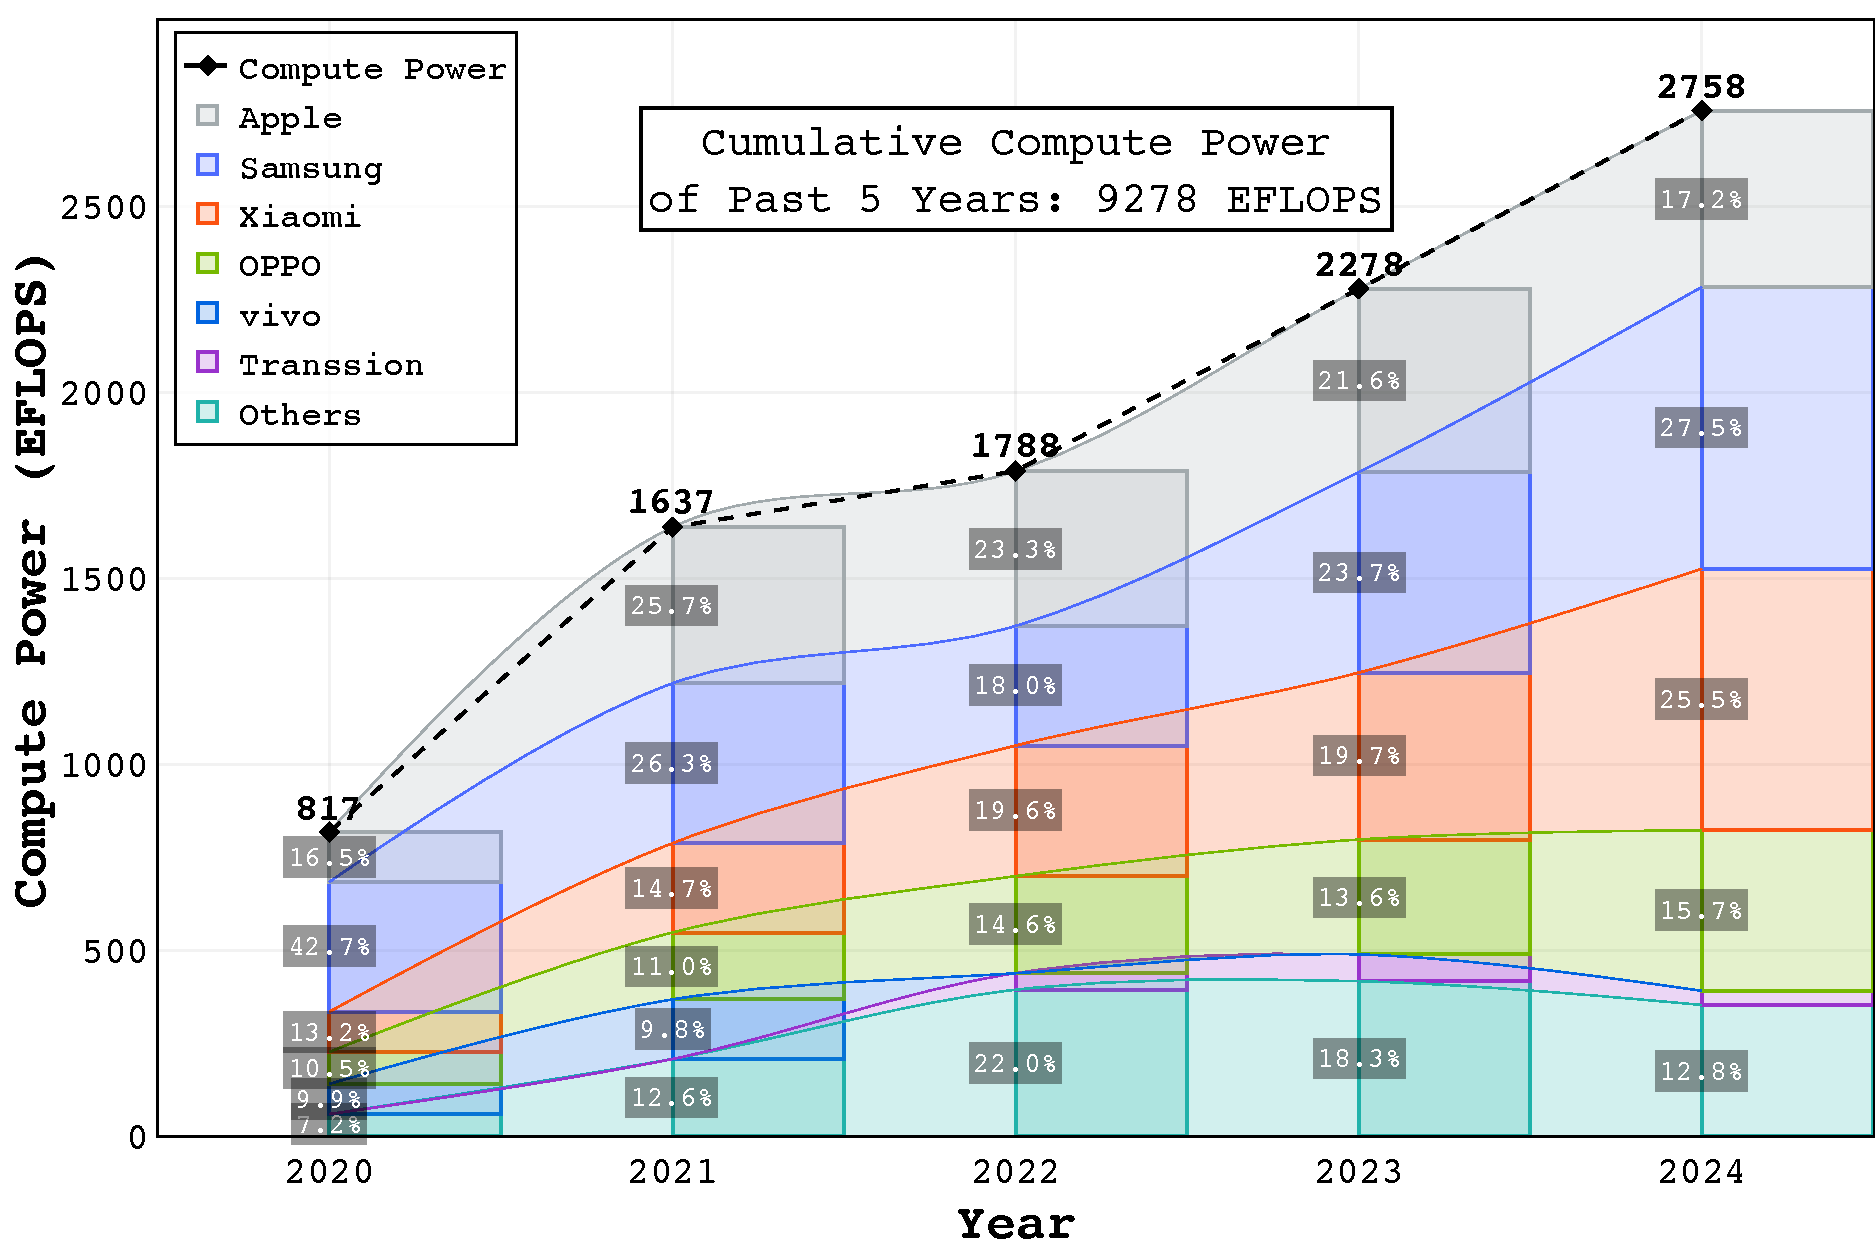
\includegraphics[width=\linewidth]{./figs/smartphone_compute_trend.pdf}
        \vspace{-20pt}
        \caption{Smartphone Market Share and Computing Power Trends. (Data source: \cite{canalys2025}).}
        \label{fig:smartphone_trend}
    \end{minipage}
\end{figure*}
\subsection{Massive Computing Power from Edges}\label{subsec:edge_compute}
% - 海量终端能提供巨大的算力
% - 单个设备(iPhone)20 TFLOPS, 单卡 200 TFLOPS,10倍。
% - Llama 算力 单卡*卡数量,TFLOPS, 得出 同等算力需要多少终端设备
% - 单个设备(iPhone)20 TFLOPS, 单卡 200 TFLOPS,10倍。
% - Llama 算力 单卡*卡数量,TFLOPS, 得出 同等算力需要多少终端设备(数字)
% - 2w 卡, 移动设备。

% 端侧算力的发展情况
% 端侧算力未来总量
% 端侧算力是否足以训练最新的模型:以Llama3和DeepSeek为例


\paragraph{Edge computing power is growing rapidly.}
In recent years, edge computing has experienced explosive growth in computing power, driving smart devices to evolve from single-function tools into multimodal perception and decision-making centers. For instance, as shown in Figure~\ref{fig:edge_trend}, flagship smartphones such as the iPhone 16 series, equipped with 3nm process chips, have achieved computing power exceeding 2 TFLOPS~\cite{apple2024iphone16pro}, enabling local execution of complex AI tasks like real-time image enhancement and multilingual speech translation. 
Notably, the computing power of an individual smartphone has potentially surpassed that of laptops in the same period.
The breakthroughs are even more pronounced in the desktop sector,
% where NVIDIA's GeForce RTX 5090, with 104.9 TFLOPS of computing power~\cite{nvidia2025}, 
achieving an annual computing power growth rate of 1.29$\times$/year, surpassing that of smartphones and laptops (both 1.20$\times$/year). 
% \footnote{{Data source: \url{https://nanoreview.net}.}}
These three types of devices form a differentiated growth hierarchy, collectively driving edge computing's overall computing power to expand at an annual average rate of 1.28$\times$/year.
% , significantly outpacing the 1.3$\times$ growth rate of cloud computing~\cite{epoch2023trendsinmachinelearninghardware}, with the gap between the two continuing to narrow. 
This growth is fueled by three key technological drivers: advanced manufacturing processes (3nm technology increases transistor density by 60\%~\cite{apple2024iphone16pro}), dedicated architectures (modern smartphone SoCs integrate NPUs for AI acceleration), and scenario-driven innovation (e.g., autonomous driving demands end-to-end latency of less than 100ms~\cite{nvidia2023}).
% The quantitative increase in computational power has led to qualitative transformations: AR/VR devices can now reduce spatial modeling latency from seconds to milliseconds~\cite{idtechex2024}; medical-grade wearable devices can perform real-time analysis of 12-lead ECG data~\cite{gopala2024}; and educational tablets are capable of rendering 8K-resolution holographic teaching environments~\cite{precedence2024}. 
% These advancements have elevated edge computing from a supporting role to a core enabler of intelligence. The rapid growth of the global edge AI chip market~\cite{cognitive2024} further underscores the trend of computing power shifting toward the edge. 
\begin{insights}
    \textbf{Insight:} 
    The smartphone computing power of the past 5 years (before 2025) is projected to reach approximately 9278 EFLOPS, with individual flagship devices now achieving over 2 TFLOPS performance. The combined parallel computing power of approximately 30 iPhone devices (with A18 chips) can match the computational capacity of a professional AI training GPU (H100 with 59.30 TFLOPS). 
\end{insights}


% \begin{table}
% \centering
% \caption{Yearly Trends in Chip Performance and Total Computing Power of Smartphone Devices. The estimation method and detailed data can be found in Appendix~\ref{app:total_computation}.}
% \vspace{0.4cm}
% \resizebox{.95\linewidth}{!}{%
% \begin{tabular}{c|c|c}
% \toprule
% \textbf{Year} & \textbf{Chip Performance Range (TFLOPS)} & \textbf{Total (EFLOPS)} \\ \midrule
% 2021 & Min: 0.24 / Median: 0.98 / Max: 1.94 & 1620 \\ \hline
% 2022 & Min: 0.25 / Median: 0.90 / Max: 1.79 & 1610 \\ \hline
% 2023 & Min: 0.23 / Median: 0.98 / Max: 2.40 & 1900 \\ \hline
% 2024 & Min: 0.33 / Median: 2.00 / Max: 2.85 & 2280 \\ \bottomrule
% \end{tabular}
% }
% \label{tab:chip_performance}
% \end{table}

\paragraph{Edge computing has potential for LLM training.}
We analyzed the performance of smartphone chips, representing typical edge devices, and estimated their overall computing power.
% , as summarized in Table~\ref{tab:chip_performance}. 
To ensure our estimation is as accurate as possible, we based our calculations on the market share data from \citet{canalys2025}.
% considering the market share distribution of different brands. 
% ToDo: 
% 1. 总算力的估计数量级算错了1140milion算成了11.4billion。
% 2. 这部分得重新算。增加出货量的图表。要得出一个总算力的数值。
% 3. intro的部分要增加总数据量和总算力的估计。
% 4. 添加引用。
% 5. 添加所有数据的table和描述。
We then estimated the total computing power of newly produced mobile devices by averaging the chip performance of each brand.
From 2020 to 2024, smartphone chip performance has seen significant improvements, with peak computing power increasing from 1.53 TFLOPS to 4.95 TFLOPS, and average computing power rising from 0.48 TFLOPS to 1.38 TFLOPS. Meanwhile, the overall computing power of mobile devices has grown from 817 EFLOPS in 2020 to 2,758 EFLOPS in 2024, and totally 9278 EFLOPS for past 5 years. This trend highlights the rapid expansion of edge computing power, which is not only essential for AI applications but also holds the potential for training complex AI models.
% For instance, training the Llama 3~\cite{meta2024llama3.1} model requires approximately 30.8 million GPU hours, equivalent to a computational demand of 1.872 million TFLOPS. If this workload were distributed across edge devices, such as the iPhone 16 series with a peak performance of 2 TFLOPS, approximately 1.547 million devices working together for one week would be sufficient to complete the training. With continuous advancements in edge chip performance and innovations like Deepseek-v3~\cite{liu2024deepseek}, which reduce computational resource consumption, large-scale collaboration of edge devices for model training is becoming increasingly feasible. As a result, the edge computing ecosystem is poised to become a key driving force for future AI innovations.
For instance, training the DeepSeek-v3~\cite{liu2024deepseek} model utilizes 2048 H100 GPUs, each providing a peak FP32 performance of 59.30 TFLOPS, resulting in a total computational capacity of 121,446.4 TFLOPS. If this workload were distributed across edge devices with a peak performance of 2 TFLOPS (e.g., mobile chips like the iPhone 16 series), approximately 60,723 users with edge devices working (\textit{ideally}) in parallel would be required to match the computational capacity. 

However, current smartphone chips are primarily optimized only for inference efficiency rather than training capabilities. 
\textit{We advocate for and predict a future trajectory of edge computing where smartphone chip designs will increasingly prioritize and optimize on-device model training capabilities.
% , fundamentally transforming the edge computing landscape.
}
As computational power grows and distributed algorithms develop, we expect a paradigm shift enabling collaborative model training across networks of edge devices. This evolution positions the edge computing ecosystem as a critical catalyst for democratizing AI development and driving the next wave of innovations in the field.



